\subsection{Apache Storm}
Apache Storm jest framworkiem umożliwiającym strumieniowe przetwarzanie danych w czasie rzeczywistym.
Charakteryzuje się przy tym:
\begin{itemize}
  \item skalowalnością,
  \item odpornością na awarię,
  \item niezawodnością.
\end{itemize}
Stworzony został przez inżynierów z firmy
Backtype \footnote{\url{https://en.wikipedia.org/wiki/BackType}},
a po jej przejęciu, rozwijany przez inżynierów Twittera \footnote{\url{https://en.wikipedia.org/wiki/Twitter}}.
Obecnie projekt jest nadzworowany przez fundację Apache \footnote{\url{https://en.wikipedia.org/wiki/Apache_Software_Foundation}}.

Podobnie jak w przypadku Apache Storm zadanie jest odseparowane od wszelkich kwestii technicznych.

Centralnym punktem jest topologia (ang. \textit{topology}),
która reprezentuje zadanie w formie acyklicznego grafu skierowanego.
Graf ten ma 2 rodzaje węzłów.
\begin{itemize}
  \item \textit{Spouts} są źródłem danych w topologii.
  Pobierają je z zewnętrznego źródła i wprowadzają wewnątrz.
  \item \textit{Bolts} są miejscem,
  w którym następuje procesowanie danych: modyfikacja, filtracja czy agregacja.
\end{itemize}
Pomiędzy węzłami poruszają się krotki (ang. \textit{tuples}),
które są kontenerami na dane wyprodukawane przez węzły.
% budowa rysunek
\begin{figure}[htbp]
\centering
	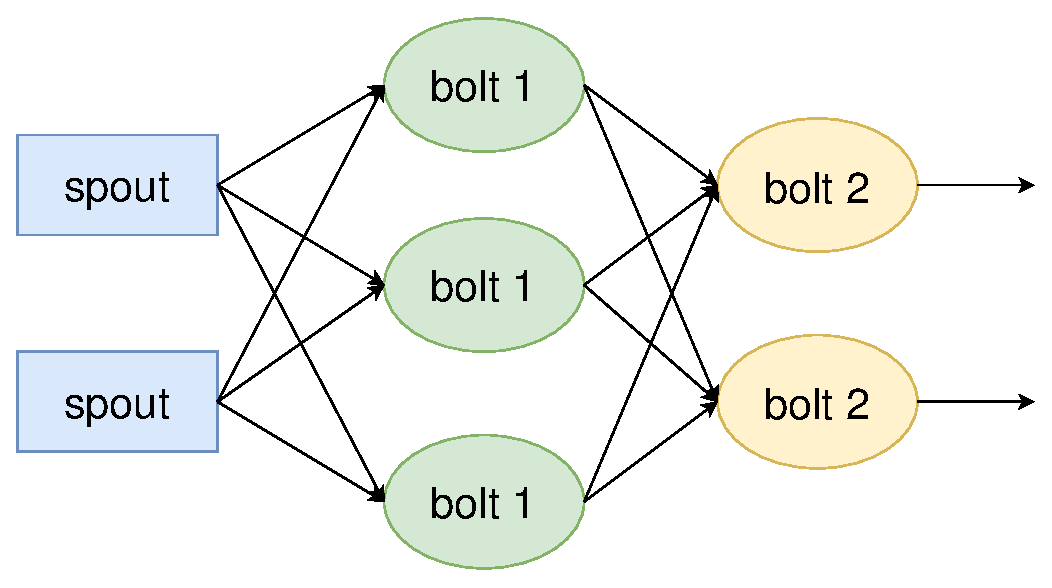
\includegraphics[width=1\textwidth]{img/storm}
	\caption{Topologia rozwiązania Apache Storm}
  \label{fig:StormTopology}
\end{figure}
% at least once
należy być przygotowanym,
że wiadomość może zostać przetworzona więcej niż jeden raz
